\documentclass[git]{deltares_manual_dfastbe}

\usepackage{tikz}
\usepackage[pipeTables=true]{markdown}
\usepackage{makecell}
%------------------------------------------------------------------------------
\newcommand{\dfastbe}{\textrm{D-FAST~Bank~Erosion}\xspace}
\newcommand{\dfbe}{\textrm{D-FAST~BE}\xspace}
\newcommand{\dflowfm}{\textrm{D-Flow~FM}\xspace}
\newcommand{\dflow}{\textrm{Delft3D-FLOW}\xspace}
\newcommand{\Frou}{\operatorname{\mathit{F\kern-.17em r}}}

% Distribution version: written by the build (CI / BuildScripts) from pyproject.toml,
% which commitizen bumps during the release workflow. Fallback keeps local compiles working.
\providecommand{\dfbeversion}{0.0.0}
\InputIfFileExists{version.tex}{}{}

\hypersetup
{
    pdfauthor   = {Deltares},
    pdftitle    = {\dfastbe},
    pdfkeywords = {Deltares User Manual \dfbe}
}

%------------------------------------------------------------------------------
%
\begin{document}
\pagestyle{empty}
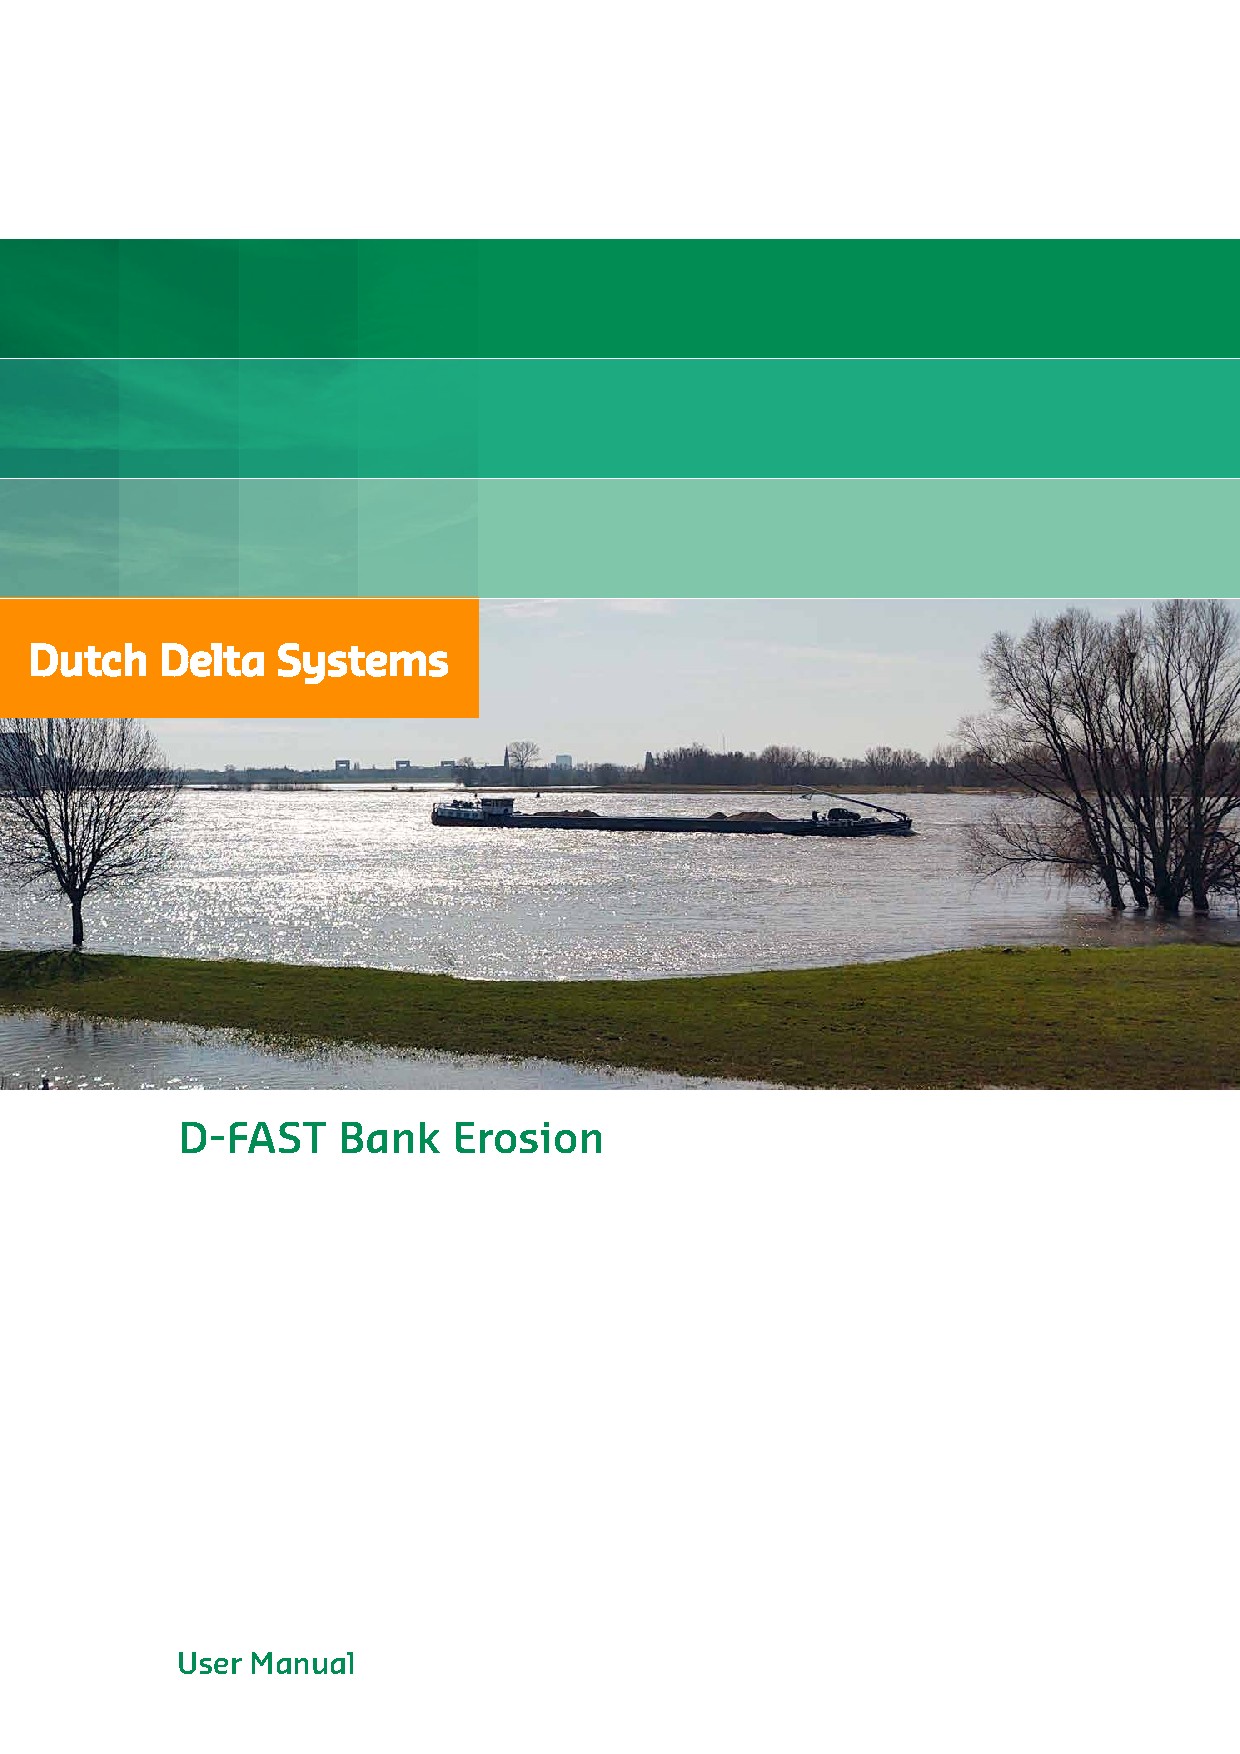
\includepdf[pages=1, offset=72 -70]{cover/D-FAST-omslag-D-FAST Bank Erosion-UM.pdf} % links-rechts past precies
\cleardoublepage
\title{D-FAST\\ Bank Erosion}
\subtitle{}
\manualtype{User Manual}
\distribution{Released for: \newline \phantom{M} \dfbe version \dfbeversion\ or higher}
\version{\the\year.\ifnum\month<10 0\fi\the\month}

\author{ }

\setgitdirectory{../.git}
\deltarestitle
%
\include{chapters/guide}
\include{chapters/introduction}
\include{chapters/get_started}
\include{chapters/detection}
\include{chapters/concepts}

\nonumchapter{References}
\bibliography{dfastbe}
%\include{chapters/references}

\appendix
\include{chapters/bankmaterial}
\include{chapters/file_formats}

\pagestyle{empty}
\cleardoublepage
\mbox{}
\includepdf[pages=2, offset=-72 -70]{cover/D-FAST-omslag-D-FAST Bank Erosion-UM.pdf} % links-rechts past precies
\end{document}
